% ============================================================
% 第 1 章 Ubuntu 与 ROS 简介
% ============================================================
% 魔术注释(供编辑器识别编译方式):
% !TEX program = xelatex
% !TEX encoding = UTF-8
% ============================================================
% 本文件有两种编译方式:
%   方式一(单独编译本章): 直接用 XeLaTeX 编译本文件, 只输出本章内容。
%   方式二(编译整本书):   编译 main.tex, 本文件会被自动 \input 引入。
% 两种方式都共用 preamble.tex, 请保持本文件与 main.tex、
% preamble.tex 位于同一目录。
% 注意: 单独编译时章编号从第 1 章重新计起, 不影响整书编号。
% ============================================================
% 单独编译开关:
%   被 main.tex 引用时, main.tex 已定义 \wholebook, 于是跳过
%   \documentclass 与导言区, 只写正文; 直接编译本文件时,
%   \wholebook 未定义, 就自动补上完整的文档头。
\ifcsname wholebook\endcsname
\else
\documentclass[12pt,a4paper]{ctexbook}
% ============================================================
% 共享导言区 preamble.tex
% 本文件被 main.tex(整书编译)和各章文件(单独编译)共同引用,
% 从而保证两种编译方式下的宏包与样式完全一致。
% 注意: 本文件不含 \documentclass, 只放宏包与样式设置。
% ============================================================
\usepackage[a4paper,margin=1.1in]{geometry}
\usepackage{graphicx}
\usepackage{listings}
\usepackage{xcolor}
\usepackage[hidelinks]{hyperref}
\usepackage{tikz}
\usetikzlibrary{positioning,arrows.meta,decorations.pathreplacing,calc}
\usepackage{booktabs}

% 代码环境样式设置
\lstset{
    basicstyle=\ttfamily\small,
    keywordstyle=\color{blue}\ttfamily,
    commentstyle=\color{gray}\ttfamily,
    stringstyle=\color{red}\ttfamily,
    backgroundcolor=\color{gray!8},
    frame=single,
    rulecolor=\color{gray!40},
    breaklines=true,
    showstringspaces=false,
    columns=fullflexible,
    keepspaces=true,
    % 允许中文注释/内容正常显示
    extendedchars=true,
    literate={
        {·}{{\cdot}}1
    }
}

\begin{document}
\fi

\chapter{Ubuntu 与 ROS 简介}

在开始敲第一行命令之前，先用一章的篇幅把两个名字弄清楚：Ubuntu 到底是什么，为什么机器人开发几乎离不开它；ROS 又是什么，为什么它叫操作系统却不是操作系统。这一章只讲概念，不讲操作，读完你就能明白后面每一章到底在做什么。

\section{什么是 Ubuntu}

\subsection{从 Linux 说起}

先纠正一个常见的误解：我们平时说的 ``Linux''，严格来讲只是操作系统的一个\emph{内核}，也就是负责管理硬件、进程、内存的那部分最核心的程序。光有内核还不足以日常使用，还需要配上图形界面、各类软件和工具，才构成一个完整可用的操作系统。内核加上这些软件的整体，叫作 Linux 的\emph{发行版}。

Ubuntu 就是众多发行版中人气最高、资料最全的一个。它基于另一个老牌发行版 Debian，由英国的 Canonical 公司维护，完全免费、开放源代码。因为用的人多，网上的教程、第三方软件、硬件驱动的支持都最齐全，所以它也是初学者最合适的入门选择。

Ubuntu 的版本号很有规律，形如 ``年份.月份''。比如 22.04 表示 2022 年 4 月发布。它每年发布两次，其中\emph{偶数年的 4 月}会发布一个特别版本，名字里带 LTS（Long Term Support，长期支持），官方会提供长达五年的维护更新。机器人开发领域几乎清一色使用 LTS 版本，图的就是稳定和长期可用，本书也以 LTS 版本为前提。

\subsection{为什么机器人开发普遍使用 Ubuntu}

机器人开发选择 Ubuntu，通常出于几个现实原因：

\begin{itemize}
    \item \textbf{ROS 官方的主战场就是 Ubuntu}。ROS 的安装、文档、示例在 Ubuntu 上支持得最好，很多版本组合甚至只有 Ubuntu 这一条 ``官方推荐'' 路线，跟着走最不容易踩坑。
    \item \textbf{免费开源}。机器人项目可以自由使用、修改和分发，不必为许可证操心。
    \item \textbf{生态成熟}。激光雷达、相机、机械臂等硬件厂商大多优先提供 Linux 驱动；论文开源代码、算法库也常在 Ubuntu 上测试。
    \item \textbf{命令行与脚本化能力强}。机器人常常需要远程登录、批量处理、自动运行，Ubuntu 的命令行环境让这些操作非常顺手。这正是第二章要练的基本功。
\end{itemize}

当然，ROS 并不是只能在 Ubuntu 上跑，其他 Linux 发行版甚至 Windows 也可以。但对新手而言，跟随 ROS 官方支持最好的 Ubuntu，能省下大量和环境搏斗的时间。
\begin{figure}[h]
  \centering
  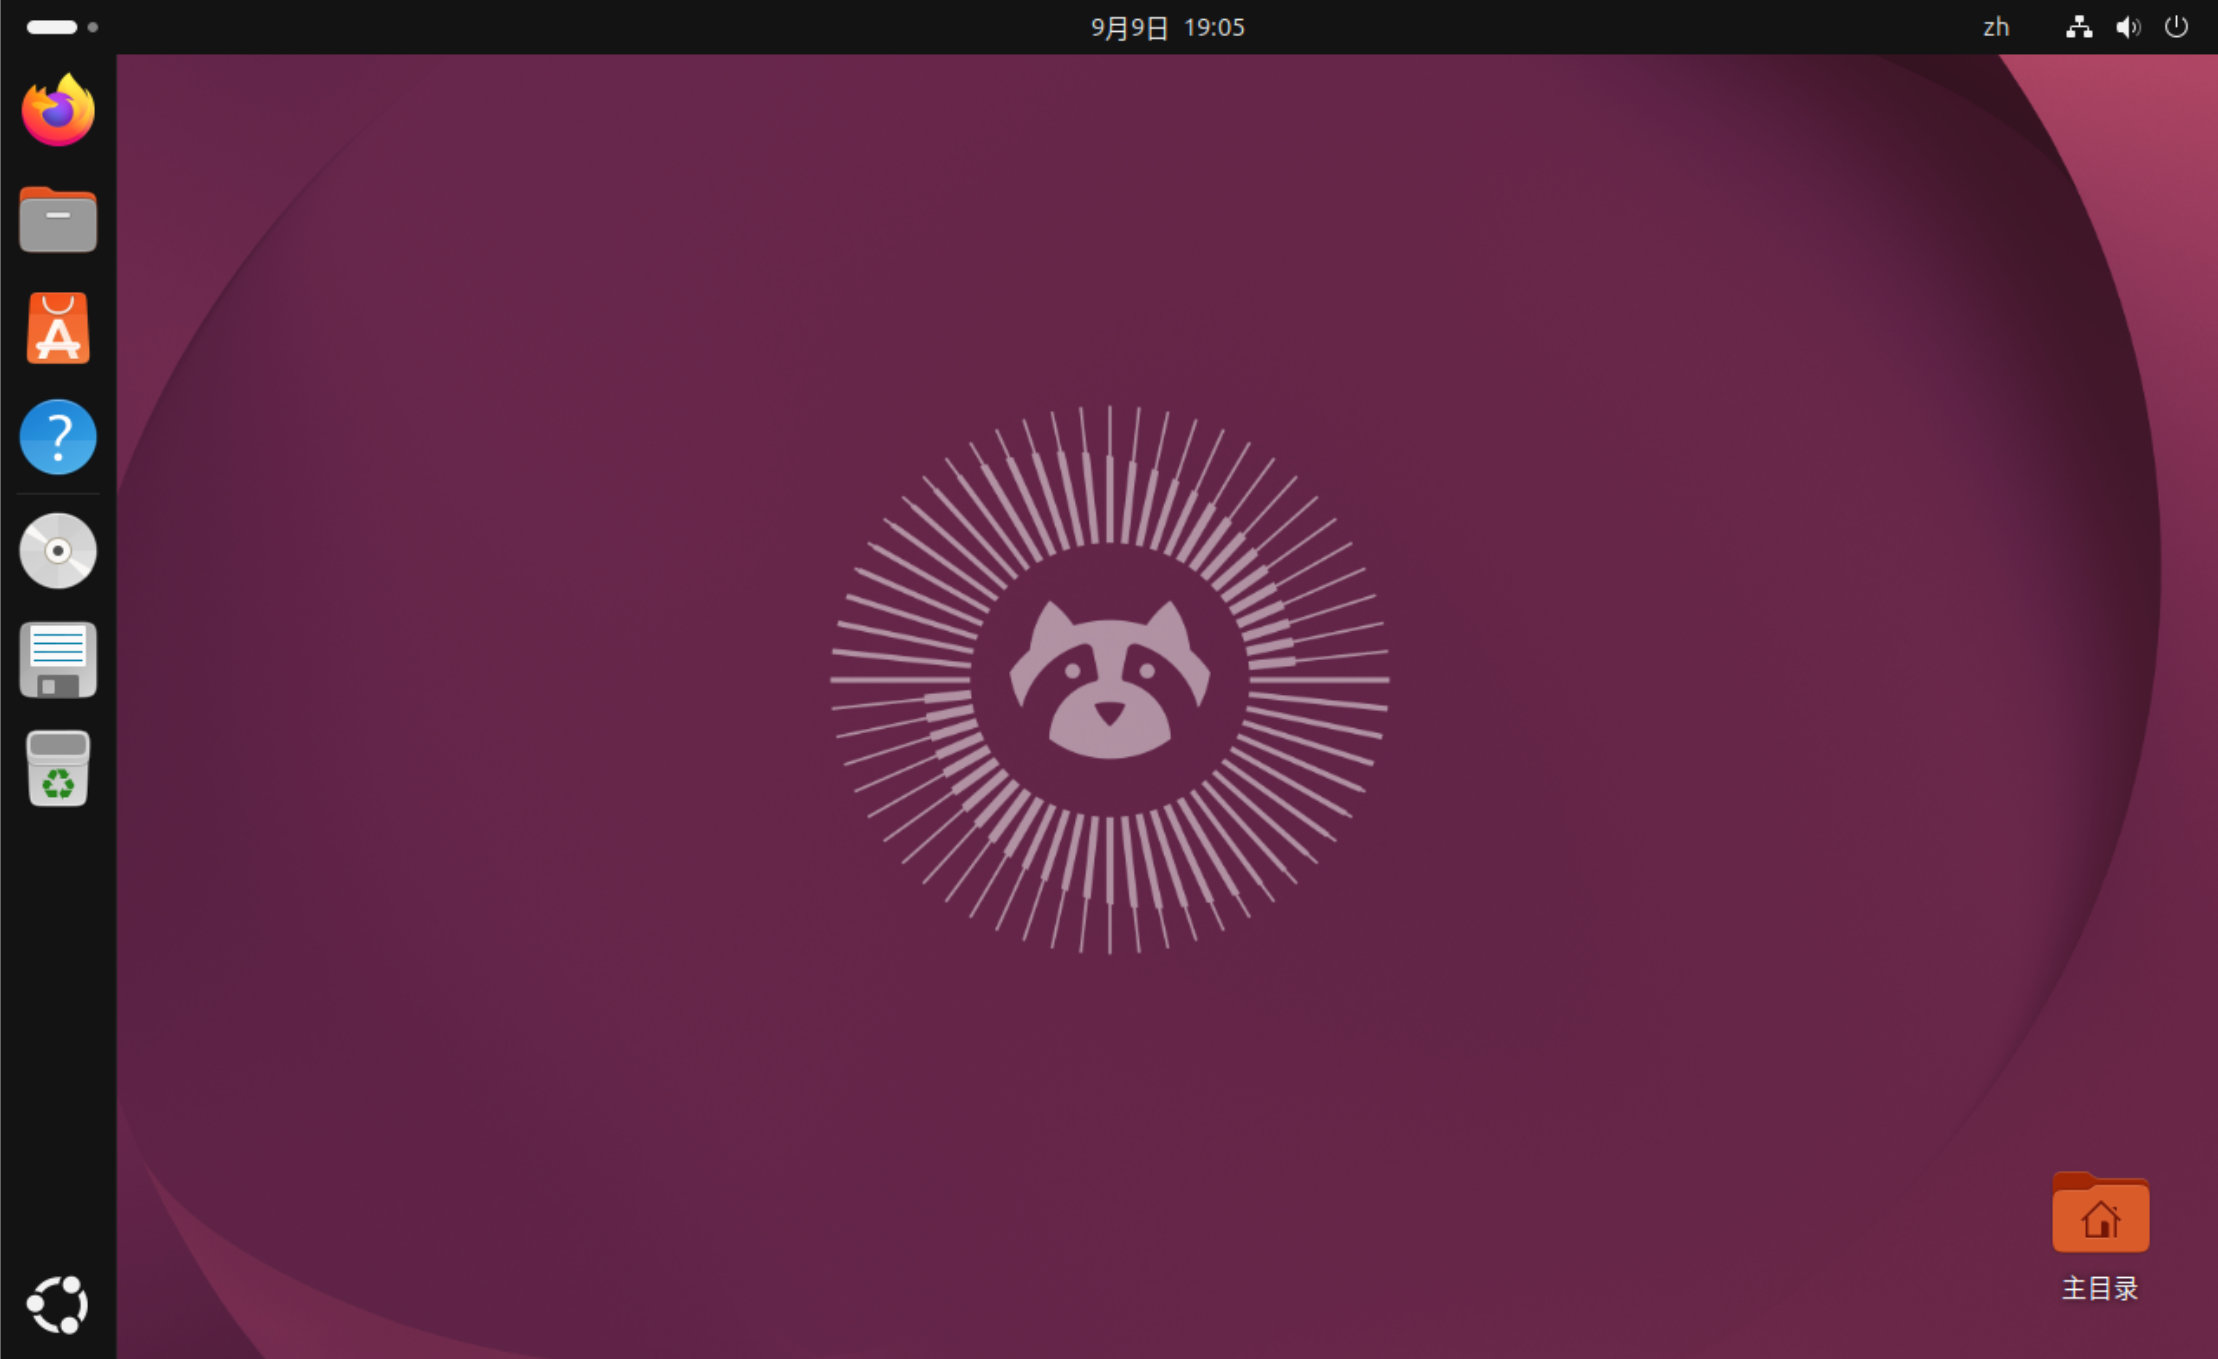
\includegraphics[width=0.8\textwidth]{Figure/Unbuntu界面.png}
  \caption{Ubuntu 桌面界面}
  \label{fig:ubuntu-desktop}
\end{figure}

\subsection{在 VMware 中安装 Ubuntu 虚拟机}

本书的最终目标，是让 ROS 2 在一套 Ubuntu 环境里跑起来。多数读者日常使用的电脑装的是 Windows，直接改装系统代价太大，因此更稳妥的起步方式是：在 Windows 里用虚拟机软件，\emph{模拟出一台完整的 Ubuntu 电脑}。虚拟机可以理解为一台由软件模拟出来的电脑，它有自己的硬盘（磁盘文件）、内存和网卡，Ubuntu 就安装在这台虚拟电脑里。这样做的好处很实在：

\begin{itemize}
    \item \textbf{不影响现有系统}。Ubuntu 只活在虚拟机窗口里，Windows 照常使用；
    \item \textbf{出错可还原}。随时可以拍摄快照，系统被折腾坏了，一键就能恢复到快照时的干净状态；
    \item \textbf{门槛低}。不用重新分区，也不涉及双系统引导，跟着下面的步骤走即可。
\end{itemize}

本小节以 VMware Workstation 为例（该软件现已对个人用户免费）。硬件上建议宿主机内存至少 8 GB，并预留 60 GB 以上的磁盘空间。

\subsubsection{准备安装材料}

需要准备两样东西：Ubuntu 系统镜像，以及 VMware Workstation 软件本身。

Ubuntu 镜像推荐使用 LTS 桌面版。官方下载地址是 \url{https://ubuntu.com/download/desktop}，如果下载速度不理想，清华（TUNA）、阿里云等国内镜像站都有完整镜像，在镜像站里找到 \url{ubuntu-releases} 目录即可。镜像文件名形如 \url{ubuntu-22.04-desktop-amd64.iso}，务必选择 \textbf{desktop}（桌面版），而不是 server（服务器版）；本书后续示例以 22.04 或 24.04 的 LTS 版本为前提。

VMware Workstation 在官网注册下载后即可免费用于个人用途，在 Windows 上按提示安装完成。

\subsubsection{在 VMware 中创建虚拟机}

打开 VMware Workstation，按照下面的步骤创建一台空白虚拟机（先不安装系统）：

\begin{enumerate}
    \item 点击主界面的\textbf{新建虚拟机}，类型选择「典型（推荐）」；
    \item 安装来源选择「\textbf{稍后安装操作系统}」。这里不要直接指定 ISO 文件，否则 VMware 会启用自动安装，反而看不到正常的安装过程；
    \item 客户机操作系统选择 \textbf{Linux}，版本选择 \textbf{Ubuntu 64 位}；
    \item 给虚拟机命名并选择存放位置；
    \item 磁盘容量建议 60 GB 以上，并选择「将虚拟磁盘拆分成多个文件」，这样日后移动、备份虚拟机都很方便；
    \item 点击「自定义硬件」：内存建议 4 GB 以上（最好 8 GB），处理器 2 核以上，网络适配器保持默认的 \textbf{NAT} 即可；
    \item 创建完成后，在左侧选中该虚拟机，打开菜单栏「虚拟机」下的「设置」，在 \textbf{CD/DVD (SATA)} 一栏勾选「启动时连接」，并浏览选择刚才下载的 Ubuntu 镜像文件，确定保存。
\end{enumerate}

\subsubsection{安装 Ubuntu 系统}

点击「开启此虚拟机」，之后的操作都发生在虚拟机窗口里：

\begin{enumerate}
    \item 从镜像引导后，在左侧语言列表选择中文（简体），点击「安装 Ubuntu」；
    \item 键盘布局保持默认即可；
    \item 在「更新和其他软件」界面，建议取消勾选「安装时下载更新」，省去漫长的等待（之后换好国内软件源再更新会快得多）；
    \item 安装类型选择「\textbf{清除整个磁盘并安装 Ubuntu}」。这一步在真实电脑上必须万分谨慎，但在虚拟机里磁盘是虚拟的，可以放心操作；
    \item 确认提示后点击「现在安装」，再点击「继续」；
    \item 时区选择 \textbf{Shanghai}，随后设置用户名和密码。\emph{请务必牢记这个密码}，之后执行 \texttt{sudo} 命令都要用到它；
    \item 等待安装完成。若屏幕提示移除安装介质后按回车，先在 VMware 菜单「虚拟机」下的「设置」里，取消 \textbf{CD/DVD (SATA)} 的「已连接」勾选，再回到虚拟机窗口按回车重启；
    \item 重启后输入密码进入桌面，Ubuntu 虚拟机就装好了。
\end{enumerate}

装好系统后先别急着开始，建议顺手完成三件事，后面能省下不少麻烦：

\begin{itemize}
    \item 安装 VMware Tools，让虚拟机与宿主机顺畅协作（见下一小节）；
    \item 更换软件源为国内镜像：打开「软件和更新」，把「下载自」的服务器改为清华或阿里镜像，之后用 \texttt{apt} 安装软件会快很多；
    \item 拍摄一张快照：在 VMware 菜单「虚拟机」下的「快照」中选择「拍摄快照」。之后系统配置坏了，随时可以恢复到当前这个干净状态。
\end{itemize}

\subsection{VMware Tools 的安装}

VMware Tools 是 VMware 提供的一组驱动和工具，装好之后虚拟机才能和宿主机顺畅协作：窗口大小自动适配分辨率、鼠标在虚拟机内外自由进出、文字可以跨系统复制粘贴、文件可以直接拖拽。过去需要在虚拟机里手动运行官方的闭源安装包，而新版 Ubuntu 完全不必如此：直接用开源的 \texttt{open-vm-tools} 即可。它由 VMware 官方推荐、随系统软件源分发，安装简单、兼容性好，还会随内核自动更新。

\subsubsection{标准安装（推荐）}

以下步骤适用于 Ubuntu 18.04 及以上版本（含 22.04、24.04）。先打开终端，更新软件包列表：

\begin{lstlisting}[language=bash,title={更新软件包列表}]
    sudo apt update
\end{lstlisting}

然后安装核心组件和桌面集成包。桌面版 Ubuntu 需要同时安装 \texttt{open-vm-tools-}\allowbreak\texttt{desktop}，它负责实现分辨率自适应、文件拖拽、复制粘贴等功能：

\begin{lstlisting}[language=bash,title={安装 open-vm-tools 及桌面集成包}]
    sudo apt install open-vm-tools open-vm-tools-desktop -y
\end{lstlisting}

安装完成后重启虚拟机，让服务生效：

\begin{lstlisting}[language=bash,title={重启虚拟机}]
    sudo reboot
\end{lstlisting}

重启回到桌面后，测试宿主机与虚拟机之间的文件拖拽、文字复制粘贴是否正常。如果一切顺利，之后在 Windows 与 Ubuntu 之间交换文件、复制命令就会非常顺手。

\subsubsection{安装失败或残留旧版时的修复}

如果之前手动安装过官方的 VMware Tools，或安装过程报错，可以先卸载清理，再重新安装：

\begin{lstlisting}[language=bash,title={卸载原有组件并清理}]
    sudo apt autoremove open-vm-tools -y
\end{lstlisting}

\begin{lstlisting}[language=bash,title={重新安装}]
    sudo apt install open-vm-tools open-vm-tools-desktop -y
\end{lstlisting}

\begin{lstlisting}[language=bash,title={重启生效}]
    sudo reboot
\end{lstlisting}

\subsubsection{传统手动安装官方 VMware Tools（不推荐）}

仅在 \texttt{open-vm-tools} 无法满足需求时，才考虑手动安装。需要说明的是，手动安装的官方工具与 \texttt{open-vm-tools} 会互相冲突，两者只能选其一；而且每次升级 Linux 内核后，官方闭源版往往需要重新安装一遍，维护成本高，所以本书不推荐这条路线。

确实需要手动安装时，步骤如下。先在 VMware 菜单栏选择「虚拟机」菜单下的「安装 VMware Tools」，虚拟机会自动挂载一个 ISO 镜像。然后进入挂载目录，把安装包拷贝到临时目录并解压：

\begin{lstlisting}[language=bash,title={拷贝安装包并解压}]
    cd /media/$USER/VMware\ Tools
    cp VMwareTools-*.tar.gz /tmp/
    cd /tmp
    tar -zxvf VMwareTools-*.tar.gz
\end{lstlisting}

接着执行安装脚本：

\begin{lstlisting}[language=bash,title={运行安装脚本}]
    cd vmware-tools-distrib
    sudo ./vmware-install.pl
\end{lstlisting}

安装过程中一路按回车接受默认配置即可，完成后重启虚拟机生效。

\section{ROS 是什么}

\subsection{ROS 不是操作系统}

ROS 的全称是 Robot Operating System，中文常译作``机器人操作系统''。这个叫法很有迷惑性：\emph{ROS 并不是一个操作系统}，它不能独立安装在裸机上，而是运行在操作系统（通常是 Ubuntu）之上的一套\emph{开源机器人软件开发框架}。

为什么机器人软件需要这样一套框架？因为一个稍微像样的机器人程序，往往由很多独立的部分组成：读取激光雷达和相机数据、处理感知、做运动规划、控制电机、与人交互……如果每个模块都自己写一套和别人通信的办法，整个系统会迅速变成一团乱麻。ROS 要解决的正是这个问题：它规定了一套统一的通信机制，并提供了大量现成的工具和功能包，让开发者可以专心写自己的那一部分，其余交给生态。

\subsection{核心概念：节点与通信}

ROS 里有两个必须最先建立印象的概念：

\begin{itemize}
    \item \textbf{节点（node）}：一个可以独立运行的程序模块。整个机器人系统可以看作许多节点协作组成的 ``网络''。
    \item \textbf{通信方式}：节点之间通过\emph{话题（topic）}、\emph{服务（service）}、\emph{动作（action）}等方式交换\emph{消息（message）}，消息就是节点间传递的数据包。
\end{itemize}

打个比方：传感器节点像是不断播报路况的广播电台（话题），导航节点像是收听广播的司机；而当你需要打车时那种``一问一答''的交互（服务），又和广播完全不同。这套通信机制的细节会在后面的章节展开，这里先记住``节点 + 通信''这个总框架即可。

\subsection{从 ROS 1 到 ROS 2}

ROS 起源于 2007 年斯坦福大学的一个机器人项目，随后由 Willow Garage 公司推动，逐渐发展成全球机器人研究界的事实标准，积累了庞大的生态。不过随着机器人应用走向工业化和复杂化，ROS 1 的一些先天设计问题开始暴露：

\begin{itemize}
    \item 通信依赖一个中心节点 \texttt{roscore}，它一旦宕机，整个系统就瘫痪；
    \item 以单机为主，多机分布式和实时性支持不足；
    \item 几乎没有安全机制，难以满足工业级要求。
\end{itemize}

于是社区从 2014 年前后开始重新设计，2017 年发布了 ROS 2 的第一个正式发行版。ROS 2 不是 ROS 1 的小修小补，而是一次架构级的重写。今天，ROS 1 已经停止维护（最后一个发行版是 2020 年的 Noetic），新项目都应当基于 ROS 2。本书讲的也是 ROS 2。

\section{ROS 1 与 ROS 2 的主要区别}

把上面的要点归纳成一张对比表，方便查阅：

\begin{center}
\begin{tabular}{|l|l|l|}
\hline
\textbf{对比项} & \textbf{ROS 1} & \textbf{ROS 2} \\
\hline
通信机制 & 自研 TCPROS/UDPROS & 基于 DDS 标准 \\
中心节点 & 依赖 \texttt{roscore} & 去中心化，无需主节点 \\
实时性 & 不支持 & 可通过 DDS 配置支持 \\
多机分布式 & 支持较弱 & 原生良好支持 \\
安全机制 & 几乎没有 & 内置（如 SROS2） \\
支持平台 & 主要 Linux & Linux/Windows/macOS 等 \\
\hline
\end{tabular}
\end{center}

对学习者而言，这些区别并不需要现在就全部弄懂。你只需要记住一个大方向：\emph{学 ROS 2}。后面章节里出现的所有命令和示例，都默认运行在 ROS 2 之上。

\section{ROS 2 与 Ubuntu 版本的搭配}

ROS 2 和 Ubuntu 一样，也有发行版的概念，而且两者高度绑定：官方每两年发布一个 ROS 2 的 LTS 版本，与当年度 Ubuntu 的 LTS 版本一一对应。最常用的组合如下：

\begin{center}
\begin{tabular}{|l|l|l|}
\hline
\textbf{Ubuntu 版本} & \textbf{ROS 2 发行版} & \textbf{说明} \\
\hline
20.04（2020 LTS） & Foxy（2020 LTS） & 较旧，资料丰富 \\
22.04（2022 LTS） & Humble（2022 LTS） & 目前最主流，教程最多 \\
24.04（2024 LTS） & Jazzy（2024 LTS） & 最新，适合新硬件 \\
\hline
\end{tabular}
\end{center}

给初学者的建议很明确：\emph{Ubuntu 22.04 + ROS 2 Humble} 是目前资料最全、社区最活跃、兼容性问题最少的组合，本书的示例也默认基于它。如果你的电脑比较新，安装 22.04 时遇到显卡或硬件驱动问题，再考虑 Ubuntu 24.04 + Jazzy 也不迟。

这里有一条最重要的原则：\emph{不要混搭}。比如在 Ubuntu 20.04 上硬装 Humble，或在 22.04 上装 Foxy，往往会遇到一堆莫名其妙的编译错误，而问题根源只是版本不对。版本搭配对了，后面能少走一半弯路。等你在第二章学会打开终端之后，可以用 \texttt{lsb\_release -a} 这条命令随时查看自己系统的 Ubuntu 版本。

\section{本书的学习路线}

这一章建立的是``地图''，接下来的章节才是``走路''：

\begin{itemize}
    \item \textbf{第二章} Ubuntu 常用指令：学会打开终端，掌握文件、目录、权限等最常用的命令，这是之后所有操作的地基；
    \item 之后是安装与配置 ROS 2，亲手把环境跑起来；
    \item 再往后深入节点、话题、服务等核心概念，配合小例子逐个验证；
    \item 最后把各部分串起来，完成小型机器人程序，体会完整的工作流。
\end{itemize}

如果你现在对 ``Ubuntu 到底是什么、ROS 能干什么'' 已经有了大致印象，那这一章的任务就完成了。翻开第二章，我们从打开终端开始。

% ============ 文件结尾 ============
% 整书模式(被 main.tex 引用): 读到这里即 \endinput 交还控制权,
% 不会执行下方的 \end{document}。
\ifcsname wholebook\endcsname
\expandafter\endinput
\fi

% 单独编译模式: 在顶层(无未闭合条件)执行 \end{document} 收尾。
\end{document}
